\documentclass[onecolumn, draftclsnofoot,10pt, compsoc]{IEEEtran}
\usepackage{graphicx}
\graphicspath{ {images/} }
\usepackage{url}
\usepackage{setspace}
\usepackage{listings}
\usepackage{color}
\usepackage{geometry}
\usepackage{float}

% For flow charts.
\usepackage{tikz}
\usetikzlibrary{shapes.geometric, arrows}

% Customizing flow chart components.
\tikzstyle{startstop} = [rectangle, rounded corners, minimum width=3cm, minimum height=1cm,text centered, draw=black, fill=red!30]
\tikzstyle{io} = [trapezium, trapezium left angle=70, trapezium right angle=110, minimum width=2cm, minimum height=1cm, text centered, draw=black, fill=blue!30]
\tikzstyle{process} = [rectangle, minimum width=3cm, minimum height=1cm, text centered, draw=black, fill=orange!30]
\tikzstyle{decision} = [diamond, minimum width=3cm, minimum height=1cm, text centered, draw=black, fill=green!30]
\tikzstyle{arrow} = [thick,->,>=stealth]



\geometry{textheight=9.5in, textwidth=7in}

\definecolor{mygreen}{rgb}{0,0.6,0}
\definecolor{mygray}{rgb}{0.5,0.5,0.5}
\definecolor{mymauve}{rgb}{0.58,0,0.82}

\lstset{
	backgroundcolor=\color{white},
	basicstyle=\footnotesize,
	captionpos=b,
	frame=single,
	keywordstyle=\color{blue},
	language=HTML,
	numbers=left,
	numberstyle=\tiny\color{mygray},
	tabsize=2
}
	
	

% 1. Fill in these details
\def \CapstoneTeamName{		Stat Champs}
\def \CapstoneTeamNumber{		59}
\def \GroupMemberOne{			Alex Hoffer}
\def \GroupMemberTwo{			Chongxian Chen}
\def \GroupMemberThree{			Jacob Smith}
\def \CapstoneProjectName{		Machine Learn Your Way to March Madness Glory}
\def \CapstoneSponsorCompany{	Oregon State University}
\def \CapstoneSponsorPerson{		Dr. Victor Hsu}

% 2. Uncomment the appropriate line below so that the document type works
\def \DocType{		%Problem Statement
				%Requirements Document
				%Technology Review
				Progress Report
				}
			
\newcommand{\NameSigPair}[1]{\par
\makebox[2.75in][r]{#1} \hfil 	\makebox[3.25in]{\makebox[2.25in]{\hrulefill} \hfill		\makebox[.75in]{\hrulefill}}
\par\vspace{-12pt} \textit{\tiny\noindent
\makebox[2.75in]{} \hfil		\makebox[3.25in]{\makebox[2.25in][r]{Signature} \hfill	\makebox[.75in][r]{Date}}}}
% 3. If the document is not to be signed, uncomment the RENEWcommand below
\renewcommand{\NameSigPair}[1]{#1}

%%%%%%%%%%%%%%%%%%%%%%%%%%%%%%%%%%%%%%%
\begin{document}
\pagenumbering{arabic}
\begin{centering}
\huge
Final Report \\
\Large 
\textbf{Name:} Alex Hoffer, Chongxian Chen, Jacob Smith \\
\textbf{Group Number:} 59 \\
\textbf{Project Title:} Machine Learn Your Way to March Madness Glory! \\
\end{centering}
%\begin{titlepage}
%\pagenumbering{gobble}
 \begin{singlespace}
   % 	\includegraphics[height=4cm]{coe_v_spot1}
    %    \hfill 
        % 4. If you have a logo, use this includegraphics command to put it on the coversheet.
        %\includegraphics[height=4cm]{CompanyLogo}   
     %   \par\vspace{.2in}
      %  \centering
 %       \scshape{
  %          \huge CS Capstone \DocType \par
   %         {\large\today}\par
    %        \vspace{.5in}
     %       \textbf{\Huge\CapstoneProjectName}\par
      %      \vfill
       %     {\large Prepared for}\par
        %    \Huge \CapstoneSponsorCompany\par
         %   \vspace{5pt}
          %  {\Large\NameSigPair{\CapstoneSponsorPerson}\par}
           % {\large Prepared by }\par
           % Group\CapstoneTeamNumber\par
            % 5. comment out the line below this one if you do not wish to name your team
         %   \CapstoneTeamName\par 
        %    \vspace{5pt}
       %     {\Large
      %          \NameSigPair{\GroupMemberOne}\par
     %           \NameSigPair{\GroupMemberTwo}\par
    %            \NameSigPair{\GroupMemberThree}\par
          %  }
   %         \vspace{20pt}
  %      }
      	 \begin{abstract}
        % 6. Fill in your abstract    
        %	This document is written using one sentence per line.
        %	This allows you to have sensible diffs when you use \LaTeX with version control, as well as giving a quick visual test to see if sentences are too short/long.
        %	If you have questions, ``The Not So Short Guide to LaTeX'' is a great resource (\url{https://tobi.oetiker.ch/lshort/lshort.pdf})
	The application of machine learning to Biochemistry and Biophysics has enabled researchers in this field to make remarkable discoveries, such as the generation of new DNA sequences. However, students of Biochemistry and Biophysics do not get the opportunity to learn machine learning. Dr. Victor Hsu of the Oregon State University Biochemistry and Biophysics department has commissioned the Stat Champs to produce an instructional module to give his students the chance to familiarize themselves with machine learning. The software product the Stats Champs have agreed to develop is a web page that allows students to train a machine learning model based on the college basketball statistics and machine learning algorithm of their choosing in order to produce a March Madness bracket. This will help students understand how machine learning algorithms produce models and how inclusion or exclusion of certain data can influence such models. Over the course of Fall term 2016, the Stat Champs developed materials such as design documents and technology reviews in order to prepare for the engineering of the module. Then, in Winter term 2017, the Stat Champs began the software development phase of this project. In Spring term 2017, the project was finished. This report comprehensively describes the lifecycle of producing the project.
      	\end{abstract}     
 	\end{singlespace}
	%\end{titlepage}
\newpage
%\pagenumbering{arabic}
\tableofcontents
% 7. uncomment this (if applicable). Consider adding a page break.
%\listoffigures
%\listoftables
\clearpage

% 8. now you write!
\section{Introduction}
Biochemistry and Biophysics are two fields that are ripe with many exciting breakthroughs. Machine learning is used by these disciplines to aid their research by providing the ability to generate new sequences of DNA. Our client, Dr. Victor Hsu, is a professor in the Biochemistry and Biophysics department at OSU who recognized that his students should understand machine learning in order to prepare them for their careers. He noticed that the department does not encourage learning machine learning, and that even if they were to, machine learning is a difficult topic for people who haven't been trained in computer science. Additionally, learning machine learning through its application to these fields can be confusing, since machine learned models of DNA can be tough to interpret. Therefore, he commissioned us to produce an online instructional module where his students could grasp machine learning fundamentals in a fun and straightforward manner. To achieve this, he asked us to provide an interface where users could select from men's college basketball statistics and generate a March Madness bracket. In doing so, budding scientists would be able to familiarize themselves with basic machine learning algorithms and also witness how the inclusion or exclusion of data influences the models trained on them. Alex Hoffer developed the GUI, Chongxian Chen implemented machine learning algorithms, and Jacob Smith gathered data for  use. Dr. Hsu's role in the project was supervision only. This report chronicles the lifecycle of the project through Fall, Winter, and Spring terms in 2017.

\section{Original Requirements Document}

\subsection{Changes from Original Requirements Document}

\section{Original Design Document}

\subsection{Changes from Original Design Document}

\section{Original Technology Review}

\subsection{Changes from Original Technology Review}

\section{Weekly Blog Posts}
\subsection{Alex}
\subsubsection{Fall Term}
\paragraph{\emph{Week 3}}
This week we collaborated with Dr. Hsu and wrote our Project Statement, which he reviewed and signed off on. We submitted the Project Statement at 11 am on 10/14/2016. We did not really encounter any problems, except for maybe some LaTek formatting issues. I am sure the use of LaTek will become easier with more practice. Next week we will be submitting our resumes for peer review and figuring out how to proceed with this project now that we have a clear, working vision to follow.
\paragraph{\emph{Week 4}}
This week we finalized our project statement by revising it to reflect our instructors' suggestions. We also all produced resumes and gave them to classmates for feedback. Next week we will work on our project requirements document and attend Career Fair.
\paragraph{\emph{Week 5}}
This week we attended career fair and developed our project requirements document. Next week we will continue developing this document and will consult the client to get his approval.
\paragraph{\emph{Week 6}}
This week we revised the rough draft of our project requirements document, formatted it using LaTek, and added a Gantt chart. We submitted this requirements document to our client, but as of 3:20 pm have not heard back from him. By the end of the weekend, we hope to have the document signed and submitted. Next week, we will individually work on our tech reviews.
\paragraph{\emph{Week 7}}
This week we revised our project requirements document and began working on our tech review document. Next week we will finish our tech review document.
\paragraph{\emph{Week 8}}
This week we developed our technology review document. We ran into some issues coming up with 3 responsibilities for everybody. We also had some difficulty identifying potential technologies for each of these responsibilities. Next week we will complete our design document.
\paragraph{\emph{Week 9}}
This week we talked about how we would make our design document, and discussed how we would approach recording ourselves for the progress report. We are having some difficulties with design document formatting. We will probably rent out a microphone for use with a computer to record ourselves for the progress report. Next week we will turn in our design document.
\paragraph{\emph{Week 10}}
This week we finished our design document. We will send it to our client and get a signature as soon as possible. We faced difficulty in getting LaTex to properly generate designs like message sequence diagrams. Next week we will submit our progress report and conclude the term.
\subsubsection{Winter Term}
\paragraph{\emph{Week 1}}
This week we came back from winter break and re-calibrated. We voted on a meeting time (Tuesdays) and attended the first class. We look forward to the term.
\paragraph{\emph{Week 2}}
This week we had our first meeting back with our TA. Our meeting consisted of planning out the term for our team. This meant we re-established the responsibilities we set for ourselves individually last term and verbally sketched out an idea of what our Beta release would look like. My own contributions this week were setting up the web page the module will be hosted on and doing some GUI work. The web page can be found here: http://web.engr.oregonstate.edu/~hoffera/CapstoneProject/MachineLearnYourWayToMarchMadnessGlory.html. More to come on the GUI work. Chongxian has set up some machine learning algorithms we can use so next week we will have Jake provide the data to them to see how they operate. After we get a handle on these algorithms, we will begin setting up the module.
\paragraph{\emph{Week 3}}
This week Chongxian arranged the machine learning algorithms, Jake compiled the statistics we'd use in a .csv file, and I worked on the GUI of our web page. Next week we have class on Thursday and wee should have the algorithms being allowed to accept stats as input.
\paragraph{\emph{Week 4}}
This week I continued to polish the GUI for the webpage. Chongxian has selected our machine learning algorithms and Jake has helped him find examples of how to implement them. Jake also gathered a lot of basketball statistics for use in the module. We need to do the OneNote portfolio, a progress report, and a voice-over update by late February.
\paragraph{\emph{Week 5}}
This week we attended class, Chongxian continued developing our machine learning algorithms, Jake continued to gather data, and I continued to develop our GUI. Next week we plan to release an alpha version of our module and we need to create a OneNote, edit our documents, make a status report, and submit these to the OneNote.
\paragraph{\emph{Week 6}}
This week we completed our progress report, both written and presentation versions. I made our OneNote and uploaded all of our documents to it. We had a bit of a hard time filling up all of the required time for the presentation. Next week we will continue development.
\paragraph{\emph{Week 7}}
This week we continued coding. I re-submitted my OneNote to Dr. Winters because it didn't go through the first time. I also met with Dr. Winters to modify my OneNote a bit. We need to finish our coding to be at a beta level release.
\paragraph{\emph{Week 8}}
This week I waited for Jake and Chongxian to make progress. Next week we need to setup a meeting with Dr. Hsu. We also are supposed to be presenting a beta release of our project.
\paragraph{\emph{Week 9}}
This week we did elevator pitches. I have made a draft of our poster using a LaTex conference poster template, and I added a signature page to our progress report and sent it to our client. My two partners should have made progress on integration. Next week I need to polish the poster more and write my new progress report, which I will use the IEEEtran format for.
\subsubsection{Spring Term}
\paragraph{\emph{Week 1}}
This week I went to class to get accustomed to what the term would entail. I updated some CSS on our page. Then, I emailed our client with a link to our project. Hope to hear from him next week and hope to update our poster for Expo.
\paragraph{\emph{Week 2}}
In week 2, Chongxian implemented different algorithms to choose from. We all updated the poster and submitted our new draft. We also emailed our client again with our finished product and our draft for him to sign off on. We await his response. In the coming weeks, we need his sign-off on the poster and then we have Expo.
\paragraph{\emph{Week 3}}
This week we attended class. I went to Dr. Hsu's office to talk to him about signing off on our posters. We also pushed our code to the Github repo. Our poster final is due May 1.
\paragraph{\emph{Week 4}}
This week I modified our poster to match our client's suggestions, then McGrath's suggestions. Then, I submitted the poster for printing. Next week I need to do the WIRED assignment.
\paragraph{\emph{Week 5}}
This week I interviewed Brandon Chatham for the WIRED assignment. We are preparing for Expo.
\paragraph{\emph{Week 6}}
This week we got our spring term progress report ready. Expo is next week and we're preparing.
\paragraph{\emph{Week 7}}
This week we had Expo. Term's almost over. In the remaining three weeks we need to edit our original docs, finish 3 small writing assignments, and do a final progress report.
\subsection{Chongxian}

\subsection{Jake}

\newpage
\section{Final Poster}
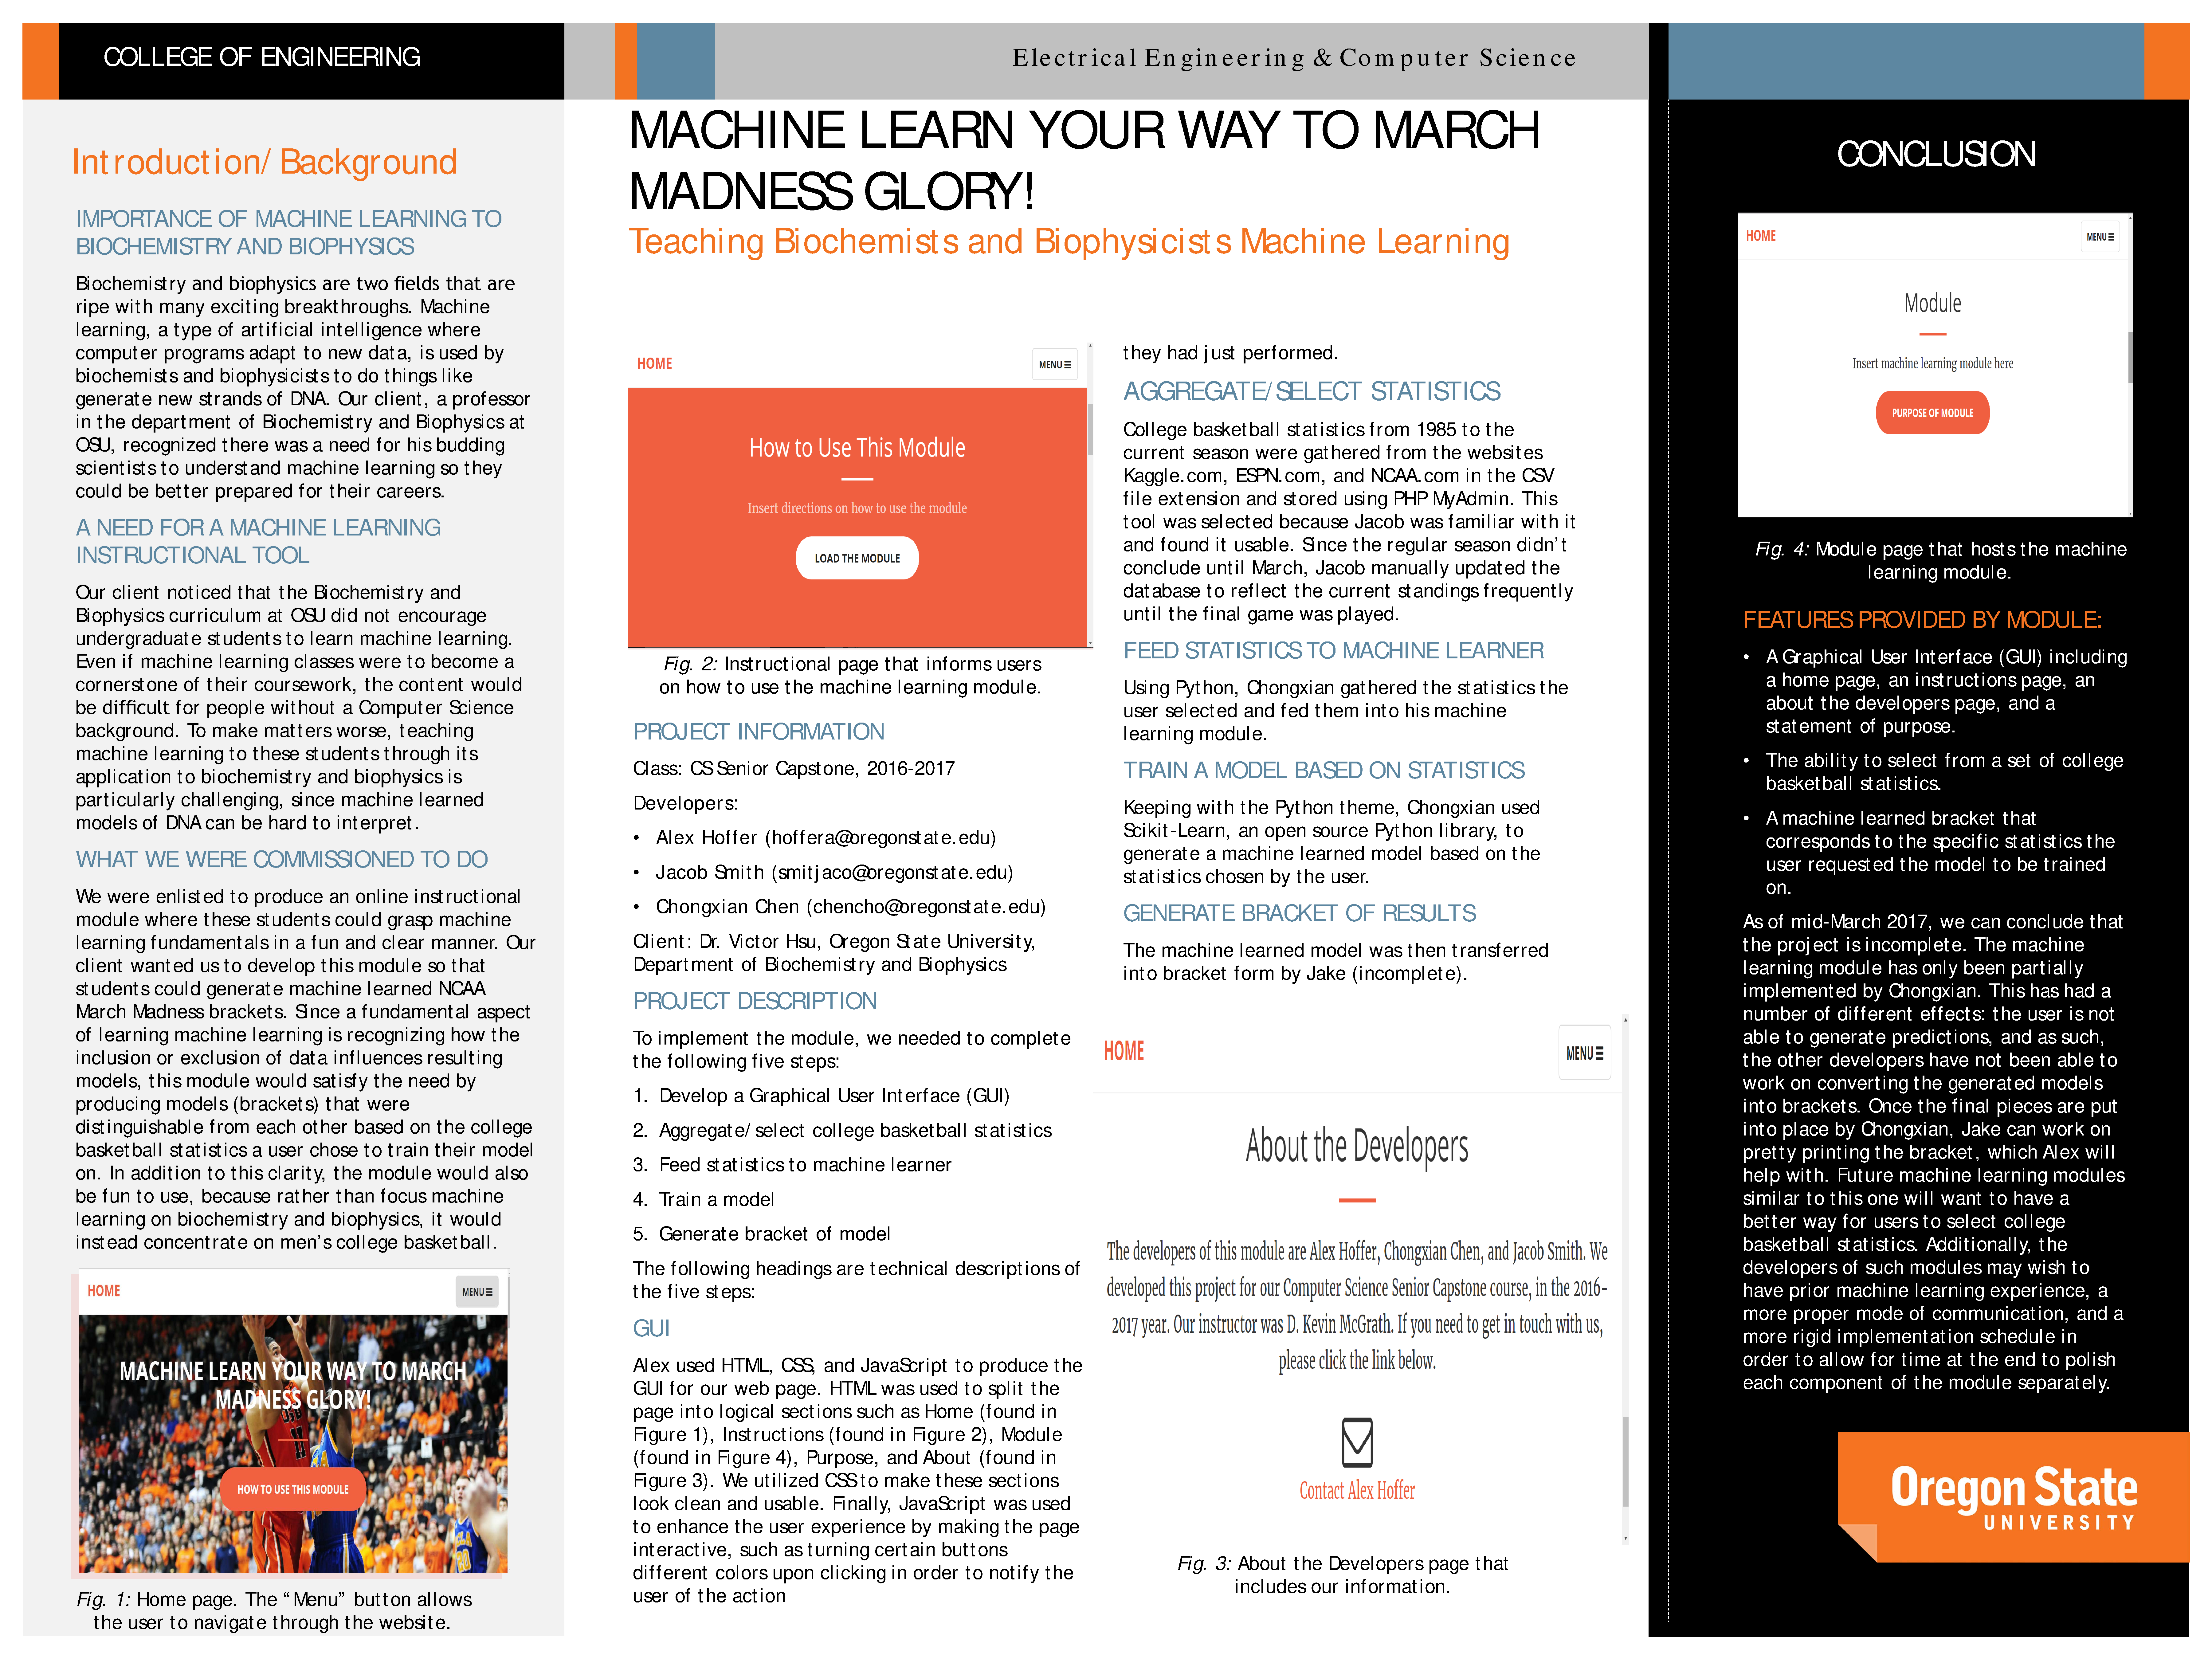
\includegraphics[width=\pagewidth,height=\pageheight,keepaspectratio]{images/Group59Poster.png}
\newpage

\section{Project Documentation}
We were both lucky and unlucky to be assigned a project that did not make well-detailed documentation a necessary responsibility. We were lucky in the sense that this shaved off a lot of work we would have to do, and unlucky in the sense that this project did not expose us to how to properly write documentation.
\subsection{How the project works}
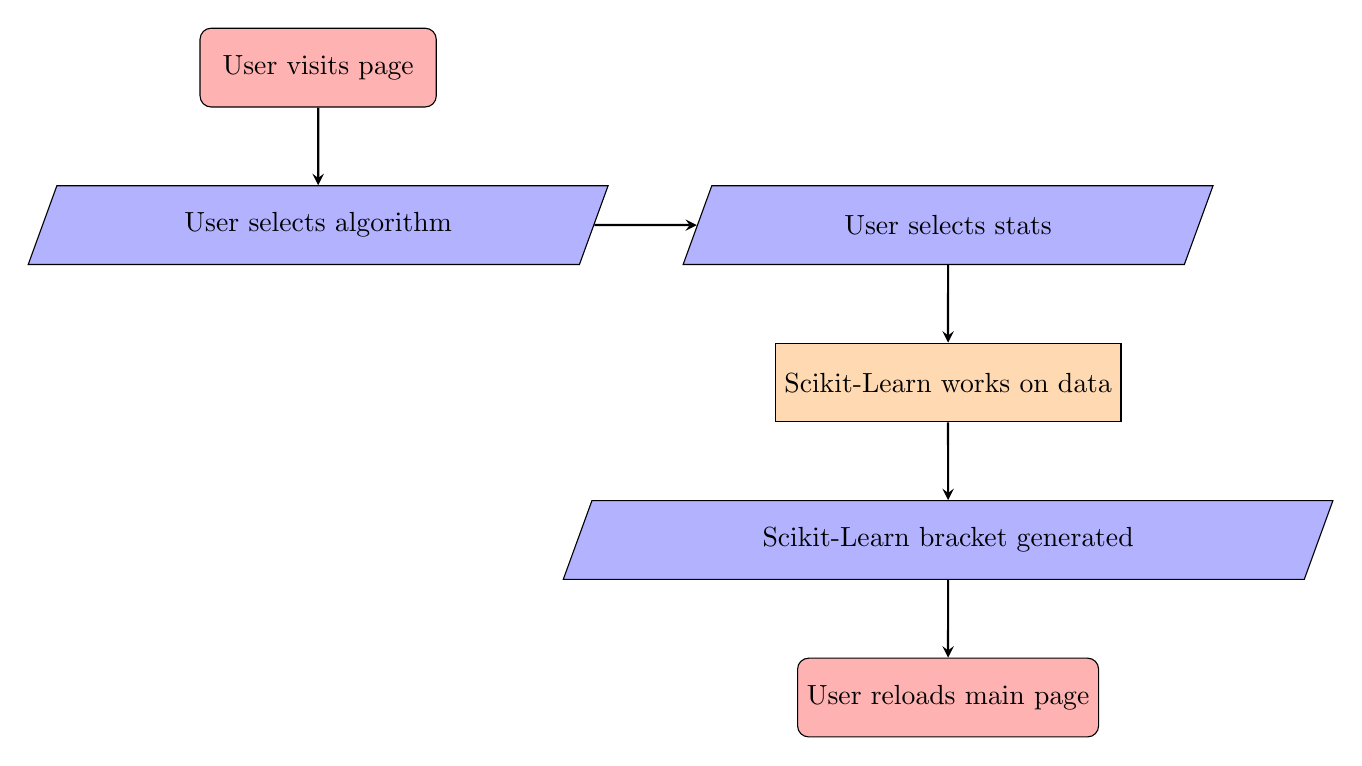
\begin{tikzpicture}[node distance=2cm]
\node (start) [startstop] {User visits page};
\node (input1) [io, below of=start] {User selects algorithm};
\node (input2) [io, right of=input1, xshift=6cm] {User selects stats};
\node (process1) [process, below of=input2] {Scikit-Learn works on data};
\node (output1) [io, below of=process1] {Scikit-Learn bracket generated};
\node (stop) [startstop, below of=output1] {User reloads main page};
\draw [arrow] (start) -- (input1);
\draw [arrow] (input1) -- (input2);
\draw [arrow] (input2) -- (process1);
\draw [arrow] (process1) -- (output1);
\draw [arrow] (output1) -- (stop);
\end{tikzpicture}

\subsection{How to use the software}
No installation is necessary. To use our software, all a user has to do is go to this website: http://web.engr.oregonstate.edu/~hoffera/CapstoneProject/MachineLearnYourWayToMarchMadnessGlory.html. On this site, a link to the machine learning module is posted. The module is compatible across all browsers. There are instructions on how to use the module on this site, as well as on the page where the module is hosted itself. To use the module, the user clicks on one machine learning algorithm and any number of the provided statistical categories and submits their choices. Then, a waiting period ranging from two minutes for simple machine learning algorithms to many hours for more precise algorithms is required. A message displays on the screen to inform the user they must wait. Then, the user is informed when the bracket has been generated. Finally, the user returns to the module page to see their generated bracket presented. The user can repeat this process an arbitrary number of times to generate an arbitrary number of brackets, but of course, the amount of time it takes to utilize certain machine learning algorithms is an important constraint the user must consider.
\subsection{Requirements for usage}
No special hardware, operating system, or runtime requirements dictate the usage of this module. As stated previously, any browser on any operating system with internet access can utilize the module.
\subsection{API Documentation}
We were not asked to document any API, and do not have any user guides. Such documents would not be particularly useful to any programmers because our module uses Scikit-Learn. This means that the API has already been documented for us by the fine people at Scikit-Learn. This documentation can be found here: http://scikit-learn.org/stable/documentation.html.

\section{How We Learned New Technology}
\subsection{Alex}
\paragraph{\emph{Websites}}
\begin{itemize}
\item https://stackoverflow.com/ 
\item https://www.w3schools.com/js/
\item http://scikit-learn.org/stable/documentation.html
\end{itemize}
Stack Overflow was most valuable because it provided useful information on debugging small issues with web development. W3 Schools was second to this, because it gave me a lot of insight on how to use JavaScript to make a website \emph{pop}. JavaScript is one of my weaker languages, so I needed it to make sure I was doing the right things. Finally, the documentation for Scikit-Learn was of course valuable for the inclusion of machine learning algorithms, but is listed last because implementation of machine learning algorithms was primarily Chongxian's responsibility.
\paragraph{\emph{People}}
Several people on campus were tremendously helpful in providing information that we needed. We owe a debt to our teaching assistant Xinze Guan for recommending Scikit-Learn for machine learning algorithm implementation. Our client, Dr. Victor Hsu, was also useful in this regard. We also relied on our instructor Kevin McGrath's LaTeX templates and Makefiles and Dr. Kirsten Winters' writing advice. Finally, my teammates helped me learn a lot of new and exciting technologies, with Jake demonstrating to me proper usage of LaTeX and Chongxian for exploring Scikit-Learn and elucidating a lot of its mysteries to me. 
\section{What We Learned}
\subsection{Alex}
\paragraph{\emph{Technical Information}}
In terms of web development, I learned more JavaScript and polished my HTML/CSS abilities. I became acquainted with how Amazon Web Services works and what their limits on their free service are. I also learned a little on how to write embedded Python, how to use Scikit-Learn in Python, and how to use Python to scrape data from websites. Since these were not my primary responsibilities, though, I didn't learn them as well as I would've liked. Finally, I learned how to use LaTeX, proper usage of the IEEETran format, and the mathematical underpinnings of various machine learning algorithms.

\paragraph{\emph{Non-Technical Information}}
I learned how to interact with a software client. I also learned how to take an idea and move it through the necessary phases of development, including requirements, planning, and design phases all the way to implementation, maintenance, and presentation. Essentially, I learned the engineering practices necessary to develop a project from embryo to adulthood, and learned how to sell or pitch an idea.
\paragraph{\emph{Project Work}}
I learned that a project must run on a well-defined schedule. If each milestone of a project builds on a previous one, this is especially important. Without a rigid schedule, you fall behind sooner rather than later and the versions of your project you will release will be fraught with bugs. 

\paragraph{\emph{Project Management}}
I learned that in a team setting, somebody has to be the team manager (whether de facto or not), otherwise milestones won't be reached and the project will be delivered late. 

\paragraph{\emph{Working in Teams}}
I discovered certain methods for overcoming differences in work style. Some people procrastinate, others get work done early. There’s nothing wrong with either approach, but if you’re in a team where there are conflicting philosophies, you need to find out early how to bridge the gap between you and your group mates.

\paragraph{\emph{What I would do differently}}
I would choose different responsibilities for this project. I wish I could’ve done more of the machine learning aspects, rather than simply oversee Chongxian’s progress. I would’ve considered using something besides Scikit-Learn  because I would’ve liked to have used more exotic machine learning algorithms, or at the very least neural networks, which are not supported in Scikit-Learn.


\subsection{Chongxian}
\subsection{Jacob}

\appendices
\section{Essential Code Listings}
\label{EssentialCodeListings}


\end{document}
